\documentclass[10pt]{article}
\usepackage{tmlr}

\input{math_commands.tex}

\usepackage{amsmath}
\usepackage{amssymb}
\usepackage{booktabs}
\usepackage{graphicx}
\usepackage{multirow}
\usepackage{placeins}
\usepackage{url}
\usepackage{hyperref}
\usepackage{xcolor}

\graphicspath{{figures/}}

\title{LASER: LAtent Space Embedding Representations for Generative Modeling}

\author{\name Anonymous Authors \email anonymous@example.com \\
      \addr Anonymous Institution}

\def\month{MM}
\def\year{2026}
\def\openreview{\url{https://openreview.net/forum?id=XXXX}}

\begin{document}

\maketitle

\begin{abstract}
Effective latent space representations are a crucial component in generative modeling. Two-stage generative models often impose structure on these representations; vector quantization is a common example, discretizing each local latent vector into one learned codebook entry. We contend that discreteness is only one possible structural choice, and that the more general principle is to impose a useful lossy compression geometry on the latent space. We propose LASER, a dictionary-learning approach that compresses latent vectors into sparse linear combinations of learned atoms, inducing a union-of-subspaces structure. To make this continuous sparse representation usable by sequential generative models, we tokenize the sparse supports and coefficient values for transformer priors. The purpose of this paper is not to claim state-of-the-art performance, but to demonstrate that sparse dictionary structure can learn compact latents and support generation. Experiments on CelebA-HQ images and VCTK raw waveform audio show that the same sparse-token interface supports reconstruction, adversarial refinement, coherent image generation, and human-sounding audio generation. These results suggest that classical signal representation ideas can provide useful alternatives to vector quantization for structuring modern generative latents.
\end{abstract}

\section{Introduction}

In generative modeling, the learning algorithm develops internal latent space representations. A common approach is to impose structure on these representations so that the downstream generative model operates on a simpler space than raw data. Vector quantization (VQ)~\citep{oord2017vqvae} is one of the most successful examples: each latent vector is mapped to a finite codebook, and the resulting indices can be modeled as discrete tokens by autoregressive priors~\citep{esser2021vqgan,vaswani2017attention}. Geometrically, VQ assumes that the latent space is well approximated by a finite set of points, inducing a Voronoi tessellation of the encoder output space.

This lossy compression approach both imposes geometric structure and provides discretization. However, these two roles need not be tied together. The geometric restriction that every latent vector must collapse to a single codebook entry can be too strict: local features cannot share or combine codebook atoms, and the model may require a larger codebook than necessary to express compositional variation. In addition, the hard assignment mechanism can underuse portions of the codebook, reducing the effective capacity of the latent space.

Realizing that quantization might not be the only answer to structuring the latent space, we separate the representation problem from the discretization problem. From a signal representation perspective, the first goal is to find a good lossy approximation to each latent vector; discretization is then an additional step that makes the representation usable by sequential generative models. LASER uses sparse dictionary learning for the first step: each latent vector or patch is represented as a sparse linear combination of learned dictionary atoms. This induces a union-of-subspaces model~\citep{olshausen1997sparse,aharon2006ksvd,tropp2007omp}, relaxing the one-code-per-site structure of VQ while retaining a compact bottleneck.

For generation, LASER converts the sparse representation into finite tokens by representing support indices and coefficient values separately. Atom indices describe which dictionary elements are active, while quantized coefficient bins describe their strengths. A transformer prior can then model these sparse codes sequentially. In this paper we instantiate this idea in a two-stage pipeline: stage 1 learns the sparse dictionary autoencoder, and stage 2 learns a spatial-depth transformer prior following the RQ-Transformer factorization~\citep{lee2022rqvae}. The stage-2 model is intentionally used as a proof of concept for sparse-code generation rather than as an exhaustive search over autoregressive architectures.

This paper makes three contributions.

\begin{itemize}
    \item A systematic perspective on latent representation learning as lossy compression, leading to a dictionary-learning bottleneck that structures latent vectors as compact sparse combinations of learned atoms.
    \item A tokenization scheme that turns real-valued sparse codes into finite support and coefficient tokens, enabling sequential generation with transformer priors.
    \item Empirical evidence on CelebA-HQ images and VCTK raw waveform audio, showing that the same sparse-token interface supports reconstruction, adversarial refinement, and generation across modalities.
\end{itemize}

The primary objective of this paper is to open the door to a wider range of approaches to improving latent space representations, rather than to claim that dictionary learning is the only useful structure or to optimize for state-of-the-art performance. We contend that the main benefit of the VQ approach comes from imposing a useful lossy compression structure on the latent space, not from discretization alone. This suggests that other classical signal representation techniques can also be useful for modern generative modeling.

\section{Structuring the Latent Space}

We consider a generic autoencoding framework with an encoder, decoder, and compression bottleneck. The encoder maps an input $x$ into a latent field $z_e$, the bottleneck produces a compressed representation $\hat{z}$, and the decoder reconstructs $\hat{x}$ from $\hat{z}$. For any local site or patch $u$, let $h_u=P_u z_e$ denote the latent vector to be compressed. In this view, the role of the bottleneck is two-fold: it should approximate the encoder latents with a simpler representation, and it should optionally discretize that representation for downstream generative modeling.

\begin{figure}[!htbp]
    \centering
    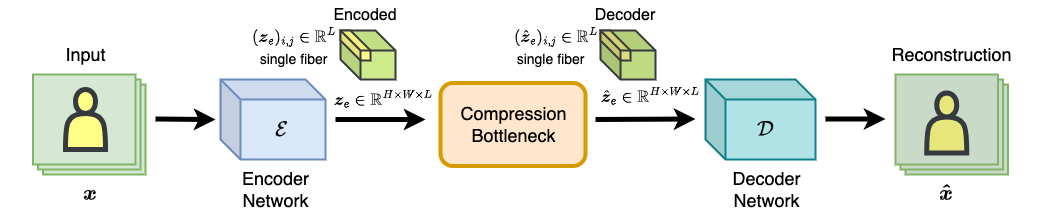
\includegraphics[width=0.84\linewidth]{generic.png}
    \caption{Generic autoencoder framework with a compression bottleneck. LASER changes the structure imposed inside this bottleneck: instead of mapping each local latent to one vector-quantized codebook entry, it represents the latent as a sparse combination of dictionary atoms.}
    \label{fig:generic-autoencoder}
\end{figure}

\subsection{Prior Approach: Vector Quantization}

Vector quantization compresses the latent space into a discrete set of learned codebook vectors. Given a codebook
\begin{equation}
    E = [e_1,\ldots,e_M] \in \mathbb{R}^{m \times M},
\end{equation}
each local latent vector $h_u$ is assigned to its nearest codebook entry:
\begin{equation}
    q(z_u=k \mid x)
    =
    \begin{cases}
        1, & k = \operatorname*{arg\,min}_{j}\|h_u-e_j\|_2,\\
        0, & \text{otherwise.}
    \end{cases}
    \label{eq:vq-assignment}
\end{equation}
The compressed latent is therefore $\hat{h}_u=e_k$ for the selected index $k$. This construction is powerful because it immediately yields integer tokens for transformer priors, but it also assumes that every local latent vector should be represented by a single prototype. LASER keeps the benefits of a compressive latent bottleneck while replacing the finite-point geometry of VQ with a union of low-dimensional subspaces.

\subsection{Our Approach: Structuring with Dictionary Learning}

Let $x \sim p_{\mathrm{data}}$ denote an image or waveform, and let an encoder produce a latent field
\begin{equation}
    z_e = E_\theta(x).
\end{equation}
We index local latent units by $u \in \mathcal{U}$. A unit can be a single latent site or a local patch, written abstractly as
\begin{equation}
    h_u = P_u z_e \in \mathbb{R}^{m},
\end{equation}
where $P_u$ extracts the local vector to be represented. LASER replaces nearest-neighbor vector quantization with a sparse dictionary code. Given normalized atoms
\begin{equation}
    D = [d_1,\ldots,d_M] \in \mathbb{R}^{m \times M}, \qquad \|d_j\|_2 = 1,
\end{equation}
each local vector is represented by a support $S_u \subset \{1,\ldots,M\}$ and coefficients $c_u \in \mathbb{R}^{|S_u|}$:
\begin{equation}
    (S_u,c_u)
    \in
    \operatorname*{arg\,min}_{S,c}
    \frac{1}{2}\|h_u - D_S c\|_2^2
    \quad \mathrm{s.t.} \quad |S| \le K .
    \label{eq:sparse-code}
\end{equation}
The sparse latent reconstruction is obtained by placing $D_{S_u}c_u$ back into the latent field:
\begin{equation}
    z_{\mathrm{sp}} = \mathcal{R}\bigl(\{D_{S_u}c_u\}_{u \in \mathcal{U}}\bigr),
\end{equation}
and the decoder models $\hat{x}=G_\psi(z_{\mathrm{sp}})$.

This bottleneck can be viewed as a union-of-subspaces generalization of a vector-quantized latent. A one-code-per-site VQ model chooses among $M$ local prototypes. LASER instead chooses one of $\sum_{k=0}^{K} {M \choose k}$ supports and then positions the vector within the selected low-dimensional subspace through $c_u$:
\begin{equation}
    D_{S_u}c_u \in \mathcal{Z}
    =
    \bigcup_{\substack{S \subseteq \{1,\ldots,M\}\\ |S|\le K}}
    \mathrm{span}\{d_j:j\in S\}.
\end{equation}
The model therefore separates \emph{which} reusable factors are active from \emph{how strongly} they are expressed. Coefficient quantization preserves this compositional structure while producing discrete tokens for a second-stage prior.

\begin{figure}[!htbp]
    \centering
    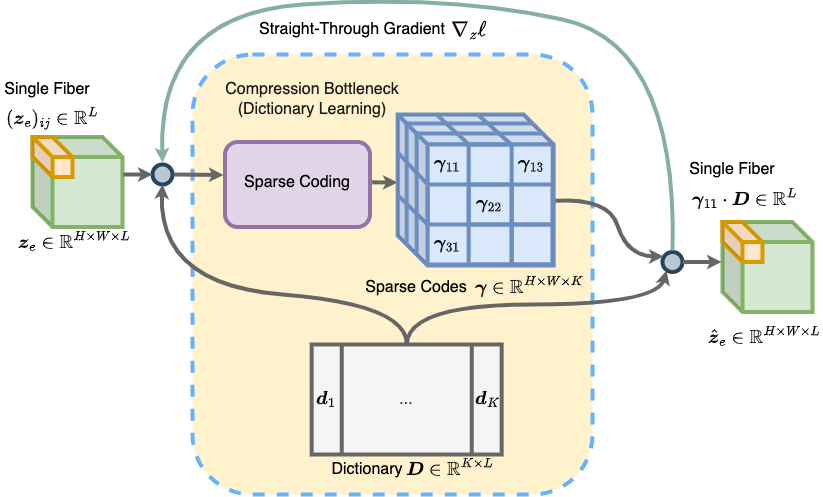
\includegraphics[width=0.76\linewidth]{dl-internal.png}
    \caption{Dictionary-learning compression bottleneck. The encoder output is sparsely coded over a learned dictionary, producing support/coefficient values that reconstruct the latent vector and can later be tokenized for generative modeling.}
    \label{fig:dictionary-bottleneck}
\end{figure}

\subsection{Training Objective}

Stage 1 is trained as an autoencoder with a sparse bottleneck. The objective is
\begin{align}
    \mathcal{L}_{\mathrm{s1}}
    =
    \mathbb{E}_{x \sim p_{\mathrm{data}}}
    \Big[
        \ell_{\mathrm{rec}}(x,\hat{x})
        + \lambda_{\mathrm{sp}}
          \sum_{u \in \mathcal{U}}\|P_u z_e - D_{S_u}c_u\|_2^2
        + \lambda_{\mathrm{coh}}\mathcal{C}(D)
    \Big],
    \label{eq:stage1-objective}
\end{align}
where $\ell_{\mathrm{rec}}$ is a modality-appropriate reconstruction loss and $\mathcal{C}(D)$ discourages degenerate dictionaries. The sparse projection is non-smooth because the support changes discretely. During autoencoder training, gradients are passed through the latent bottleneck with a straight-through estimator, so the decoder is trained on sparse latents while the encoder receives reconstruction signal.

For images, $\ell_{\mathrm{rec}}$ combines pixel and perceptual reconstruction terms when enabled. For raw waveform audio, it combines waveform and spectral reconstruction terms. These choices affect the metric surface but not the latent variable factorization in Eq.~\ref{eq:sparse-code}.

As in adversarial autoencoding and VQGAN-style training, the reconstruction objective can be augmented with a discriminator loss to improve perceptual sharpness. In that case, the encoder, dictionary bottleneck, and decoder define the generator, while a patch discriminator distinguishes real samples from reconstructions. This adversarial extension changes the training signal but leaves the sparse latent representation and tokenization unchanged.

\begin{figure}[!htbp]
    \centering
    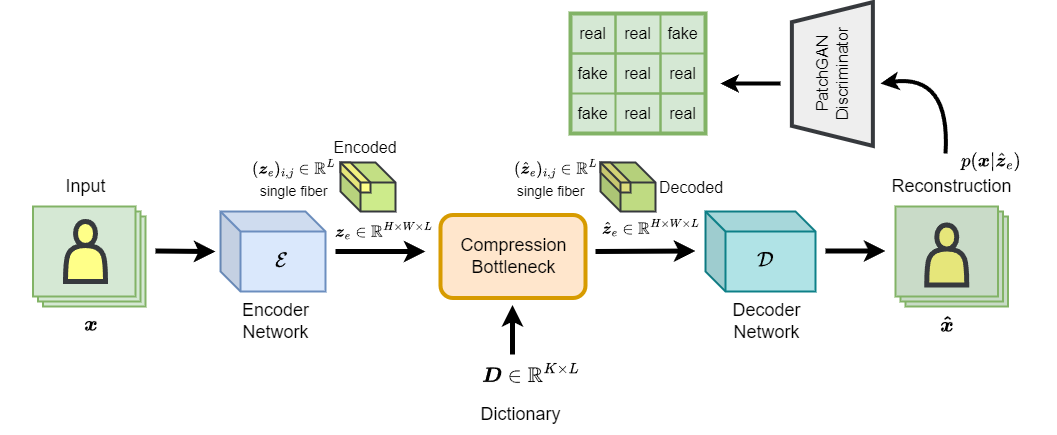
\includegraphics[width=0.88\linewidth]{dlgan-arch.png}
    \caption{Adversarial extension of the dictionary-learning autoencoder. A patch discriminator supplies an additional perceptual training signal while the compression bottleneck remains the sparse dictionary representation.}
    \label{fig:dlgan-arch}
\end{figure}

\subsection{Tokenization}

For generative modeling, each sparse code must be converted into a sequence. The unordered support in Eq.~\ref{eq:sparse-code} is first canonicalized by sorting atom ids. With $K$ active slots and quantized coefficients, the token tuple for unit $u$ is
\begin{equation}
    y_u =
    [i_{u,1}, b_{u,1}, i_{u,2}, b_{u,2}, \ldots, i_{u,K}, b_{u,K}],
    \label{eq:sparse-token}
\end{equation}
where $i_{u,k}$ is an atom id and $b_{u,k}=Q(c_{u,k})$ is a coefficient-bin id. Let $\tilde{c}_u$ denote the dequantized coefficient vector recovered from these bins. If the coefficient quantizer has step size $\Delta$, the local quantization perturbation satisfies
\begin{equation}
    \|D_{S_u}(c_u-\tilde{c}_u)\|_2
    \le
    \|D_{S_u}\|_2 \frac{\sqrt{K}\Delta}{2}.
\end{equation}
Thus coefficient resolution controls a direct bound on local latent distortion, while the support controls the discrete combinatorial part of the representation.

The resulting sparse-token grid is denoted
\begin{equation}
    Y \in \{1,\ldots,V\}^{H_c \times W_c \times D_t},
\end{equation}
where $D_t=2K$ for quantized coefficients. In real-valued variants, atom ids remain discrete while coefficients are modeled as continuous values; the experiments in this paper use quantized coefficients.

\subsection{Prior Modeling with a Spatial-Depth Transformer}

The second stage follows the theoretical factorization of RQ-Transformer~\citep{lee2022rqvae}, adapted from residual-quantized code stacks to LASER sparse-token tuples. Let $T=H_cW_c$ and rearrange the spatial indices of $Y$ in raster-scan order to obtain
\begin{equation}
    S \in \{1,\ldots,V\}^{T \times D_t},
    \qquad
    S_t=(S_{t,1},\ldots,S_{t,D_t}),
\end{equation}
where $S_t$ is the ordered support/coefficient token stack at spatial position $t$. The autoregressive prior is factorized as
\begin{equation}
    p(S)
    =
    \prod_{s=1}^{T}
    \prod_{d=1}^{D_t}
    p(S_{s,d} \mid S_{<s}, S_{s,<d}),
    \label{eq:spatial-depth}
\end{equation}
where $S_{<s}$ denotes all token stacks at earlier raster positions and $S_{s,<d}$ denotes earlier tokens in the current stack. This matches the RQ-Transformer view that generation should predict the next stack of local latent codes rather than flattening the entire $T D_t$ grid into an undifferentiated sequence.

The spatial transformer summarizes information from previous positions. Let $e(\cdot)$ be a learned token embedding and $p^{\mathrm{sp}}_t$ be a spatial positional embedding. We embed the previous sparse-token stack as
\begin{equation}
    u_t = p^{\mathrm{sp}}_t + \sum_{d=1}^{D_t} e(S_{t-1,d}), \qquad t>1,
\end{equation}
with $u_1$ represented by a learned start embedding. A causal spatial transformer maps $(u_1,\ldots,u_t)$ to a context vector $h_t$ that encodes $S_{<t}$.

Given $h_t$, the depth transformer predicts the tokens inside the current sparse tuple. With depth positional embeddings $p^{\mathrm{dep}}_d$, its inputs are
\begin{equation}
    v_{t,1}=p^{\mathrm{dep}}_1+h_t,\qquad
    v_{t,d}=p^{\mathrm{dep}}_d+\sum_{d'=1}^{d-1}e(S_{t,d'}),\quad d>1.
\end{equation}
A causal depth transformer over $(v_{t,1},\ldots,v_{t,d})$ outputs the conditional distribution
\begin{equation}
    p_{t,d}(\cdot)
    =
    p(S_{t,d}=\cdot \mid S_{<t},S_{t,<d}),
\end{equation}
and the stage-2 objective is the negative log-likelihood
\begin{equation}
    \mathcal{L}_{\mathrm{AR}}
    =
    \mathbb{E}_{S}\left[
    -\sum_{t=1}^{T}\sum_{d=1}^{D_t}
    \log p(S_{t,d}\mid S_{<t},S_{t,<d})
    \right].
\end{equation}

This decomposition matches the semantics of the LASER latent code: spatial positions carry global image or audio arrangement, while depth positions describe the local sparse mixture through support and coefficient tokens. It also inherits the computational motivation of RQ-Transformer. A naive transformer over a length-$TD_t$ sequence has attention cost quadratic in $TD_t$, whereas separating the spatial and depth transformers gives costs governed by a length-$T$ spatial sequence and length-$D_t$ depth sequences.

\subsection{Cross-Modal View}

The same construction applies to image and waveform data. Images use local two-dimensional latent patches. Audio uses temporal latent patches produced from raw waveform segments. The decoder and reconstruction loss are modality-specific, but the latent variable in Eq.~\ref{eq:sparse-code}, the tokenization in Eq.~\ref{eq:sparse-token}, and the prior factorization in Eq.~\ref{eq:spatial-depth} are shared.

\FloatBarrier

\section{Experiments}

\subsection{Detailed Experimental Setup}

The experiments focus on one image setting and one audio setting. The image setting is CelebA-HQ at $256 \times 256$ with non-overlapping $2 \times 2$ latent patches, sparsity $K=4$, and 256 coefficient bins. The audio setting is VCTK raw waveform modeling with the same patch size, stride, sparsity, and coefficient quantization. In both settings, stage 1 learns the sparse dictionary autoencoder and stage 2 learns the spatial-depth prior over the resulting sparse-token grid.

\subsection{CelebA-HQ Image Results}

Table~\ref{tab:celeb-stage1} reports CelebA-HQ stage-1 reconstruction FID for the non-adversarial checkpoint and the adversarial continuation. The adversarial continuation improves rFID from 29 to 16.

\begin{table}[!htbp]
\centering
\small
\caption{CelebA-HQ $256 \times 256$ stage-1 reconstruction FID for the reported LASER instance. Lower is better.}
\label{tab:celeb-stage1}
\begin{tabular}{lr}
\toprule
Checkpoint & rFID \\
\midrule
Non-adversarial & 29 \\
Adversarial & 16 \\
\bottomrule
\end{tabular}
\end{table}

The stage-1 media in Figures~\ref{fig:celebahq-stage1-noadv-grid},~\ref{fig:celebahq-stage1-adv-grid}, and~\ref{fig:celebahq-stage1-helpers} show validation reconstructions and sparse-code diagnostics for both the non-adversarial checkpoint and the adversarial continuation.

\begin{figure}[!htbp]
    \centering
    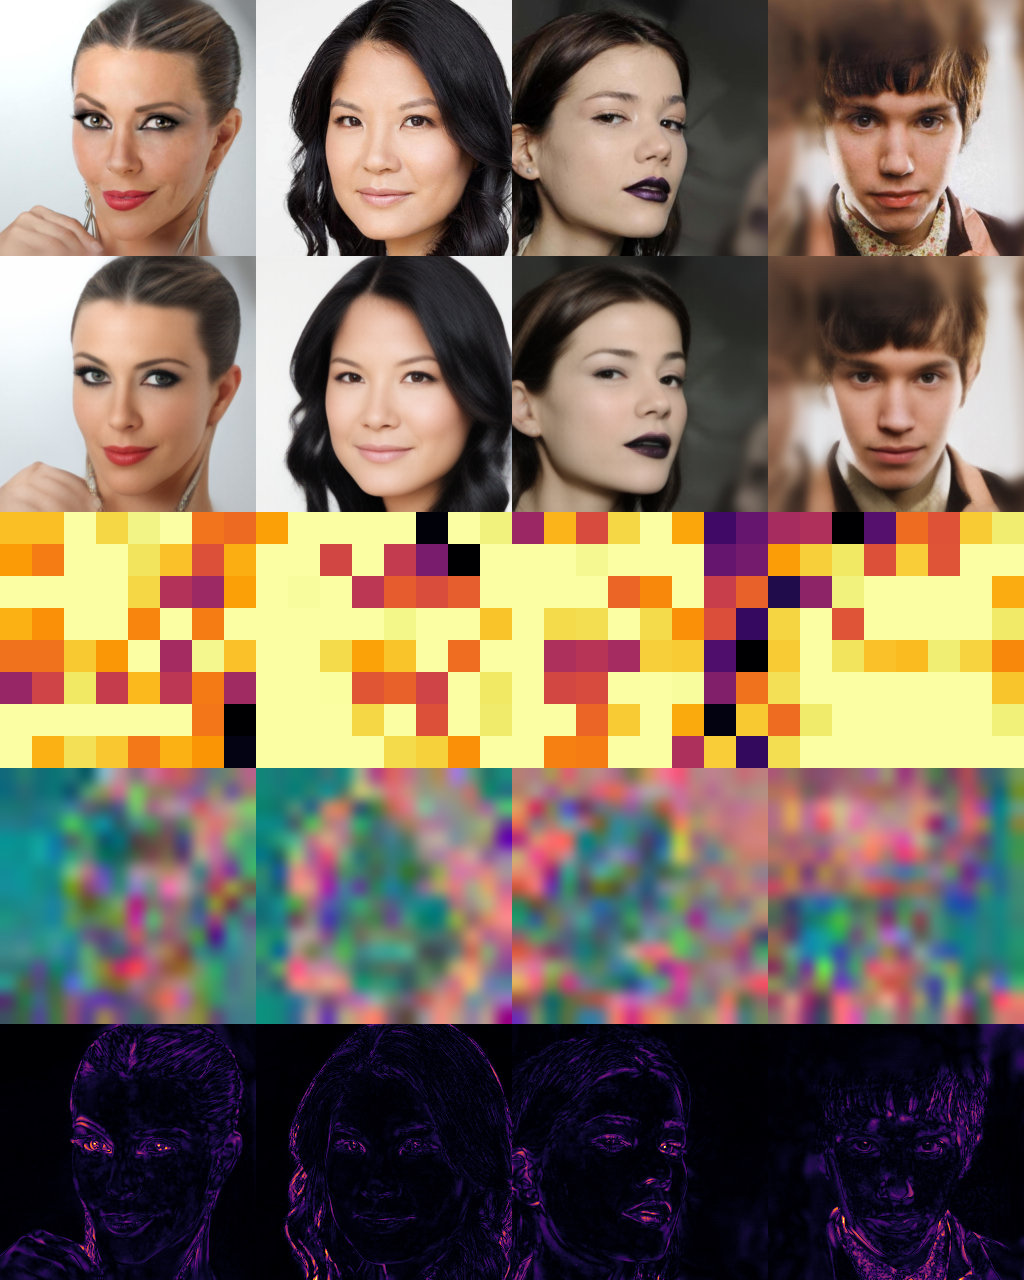
\includegraphics[width=0.82\linewidth]{celebahq_stage1_noadv_validation_grid.png}
    \caption{CelebA-HQ non-adversarial stage-1 validation diagnostics for four examples. Rows are original images, reconstructions, sparse heatmaps, latent RGB helpers, and reconstruction error maps.}
    \label{fig:celebahq-stage1-noadv-grid}
\end{figure}

\begin{figure}[!htbp]
    \centering
    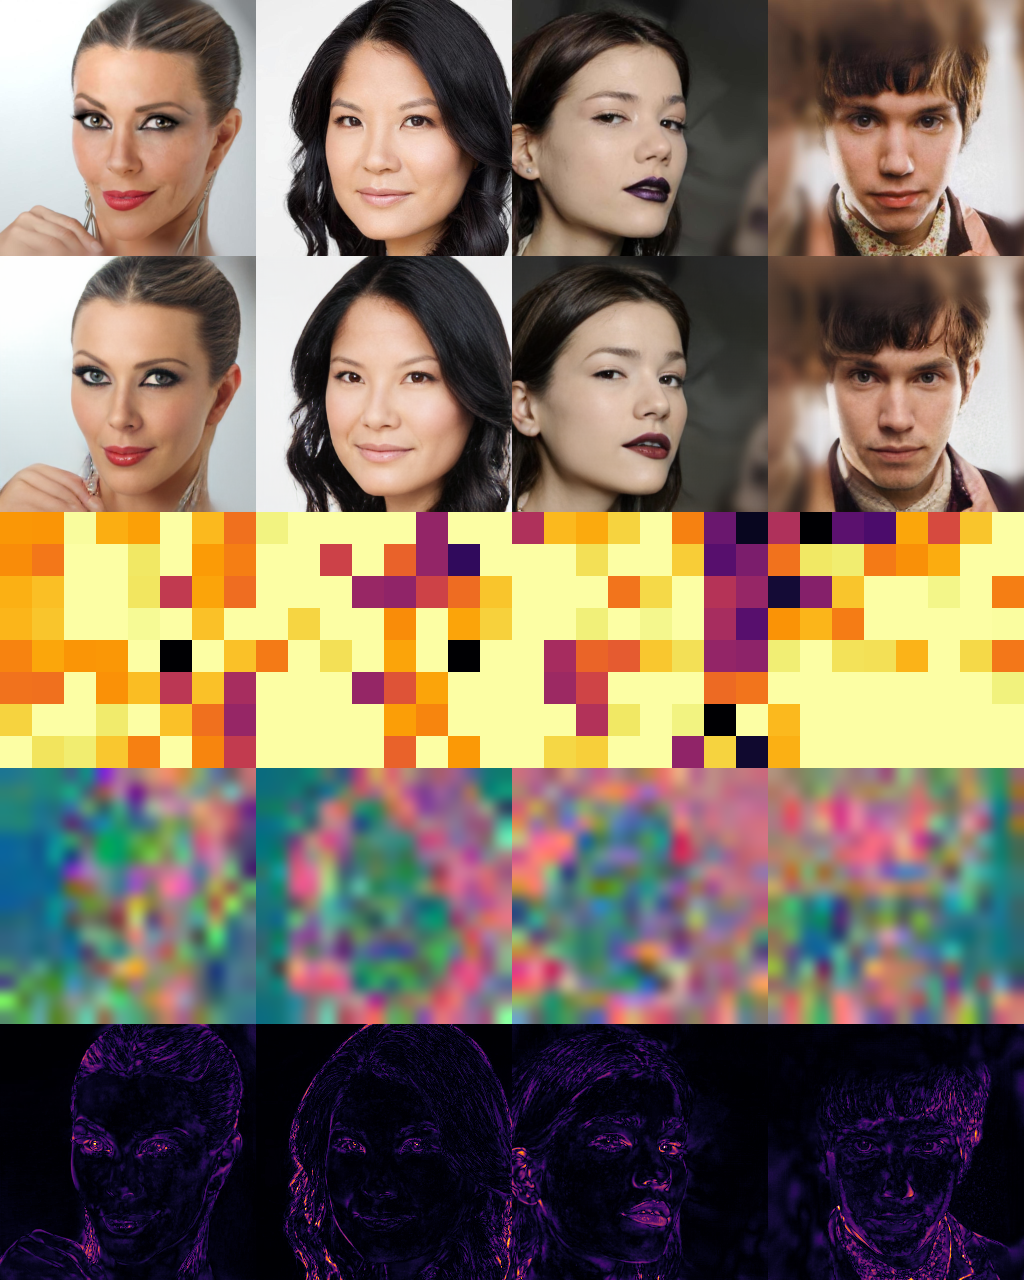
\includegraphics[width=0.82\linewidth]{celebahq_stage1_adv_validation_grid.png}
    \caption{CelebA-HQ adversarial stage-1 validation diagnostics for the same four examples. Rows are original images, reconstructions, sparse heatmaps, latent RGB helpers, and reconstruction error maps.}
    \label{fig:celebahq-stage1-adv-grid}
\end{figure}

\begin{figure}[!htbp]
    \centering
    \small
    \begin{tabular}{cc}
        Latent RGB & Dictionary scatter \\
        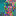
\includegraphics[width=0.28\linewidth]{celebahq_stage1_noadv_latent_rgb.png} &
        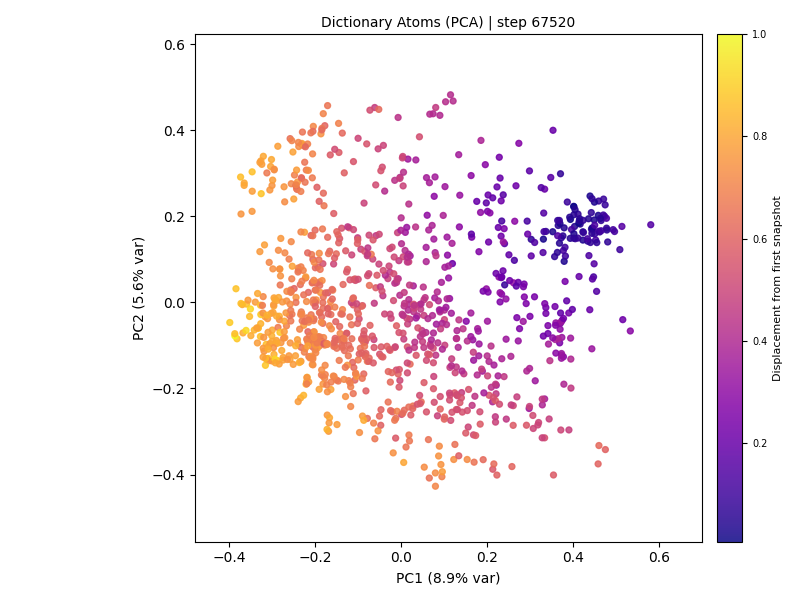
\includegraphics[width=0.58\linewidth]{celebahq_stage1_noadv_dictionary_scatter.png} \\
        \multicolumn{2}{c}{Non-adversarial stage 1} \\
        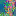
\includegraphics[width=0.28\linewidth]{celebahq_stage1_adv_latent_rgb.png} &
        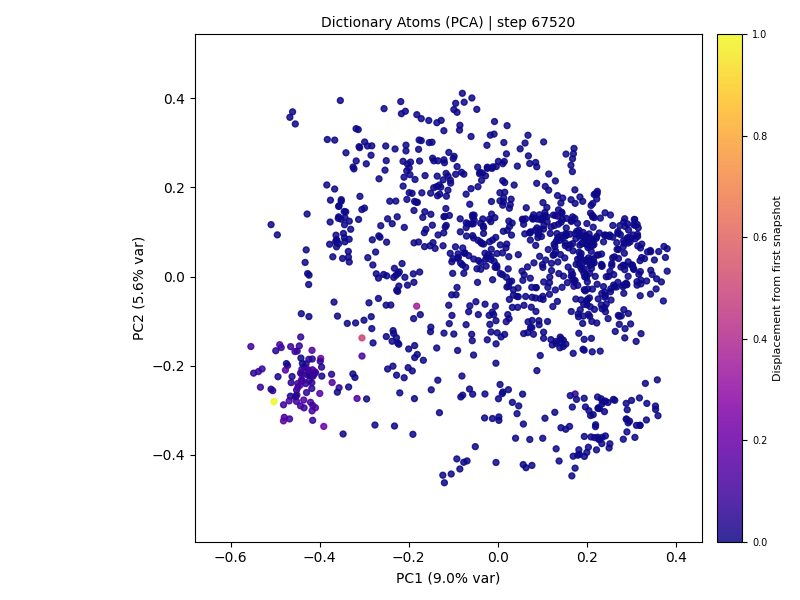
\includegraphics[width=0.58\linewidth]{celebahq_stage1_adv_dictionary_scatter.png} \\
        \multicolumn{2}{c}{Adversarial stage 1}
    \end{tabular}
    \caption{Additional CelebA-HQ stage-1 helper visualizations for the selected non-adversarial and adversarial checkpoints.}
    \label{fig:celebahq-stage1-helpers}
\end{figure}

The corresponding stage-2 prior is trained on the quantized sparse-token grid from this setting. We report its output qualitatively through decoded sample crops, since the central question is whether the sparse-token prior can produce coherent face samples through the learned dictionary decoder.

\begin{figure}[!htbp]
    \centering
    \begin{tabular}{cc}
        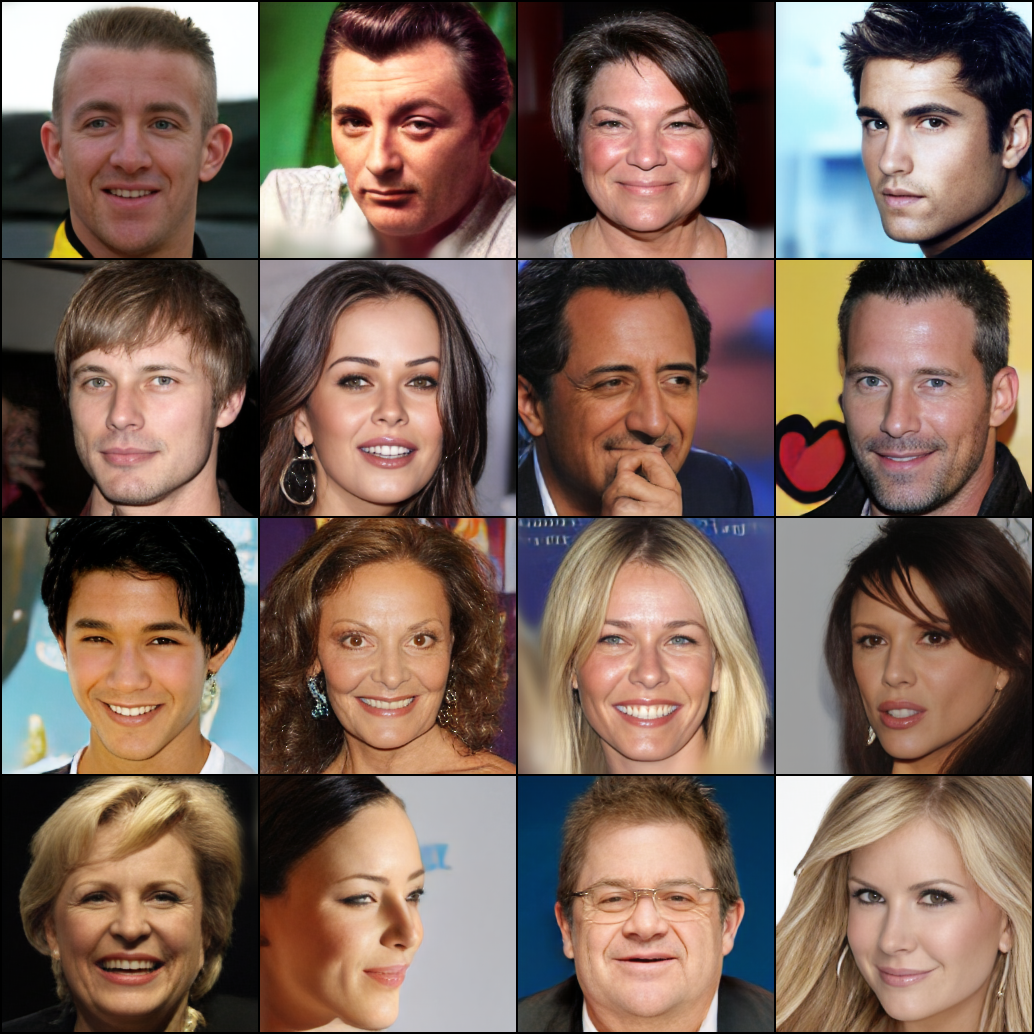
\includegraphics[width=0.47\linewidth]{celebahq_powerlong_stage2_samples_4x4_01.png} &
        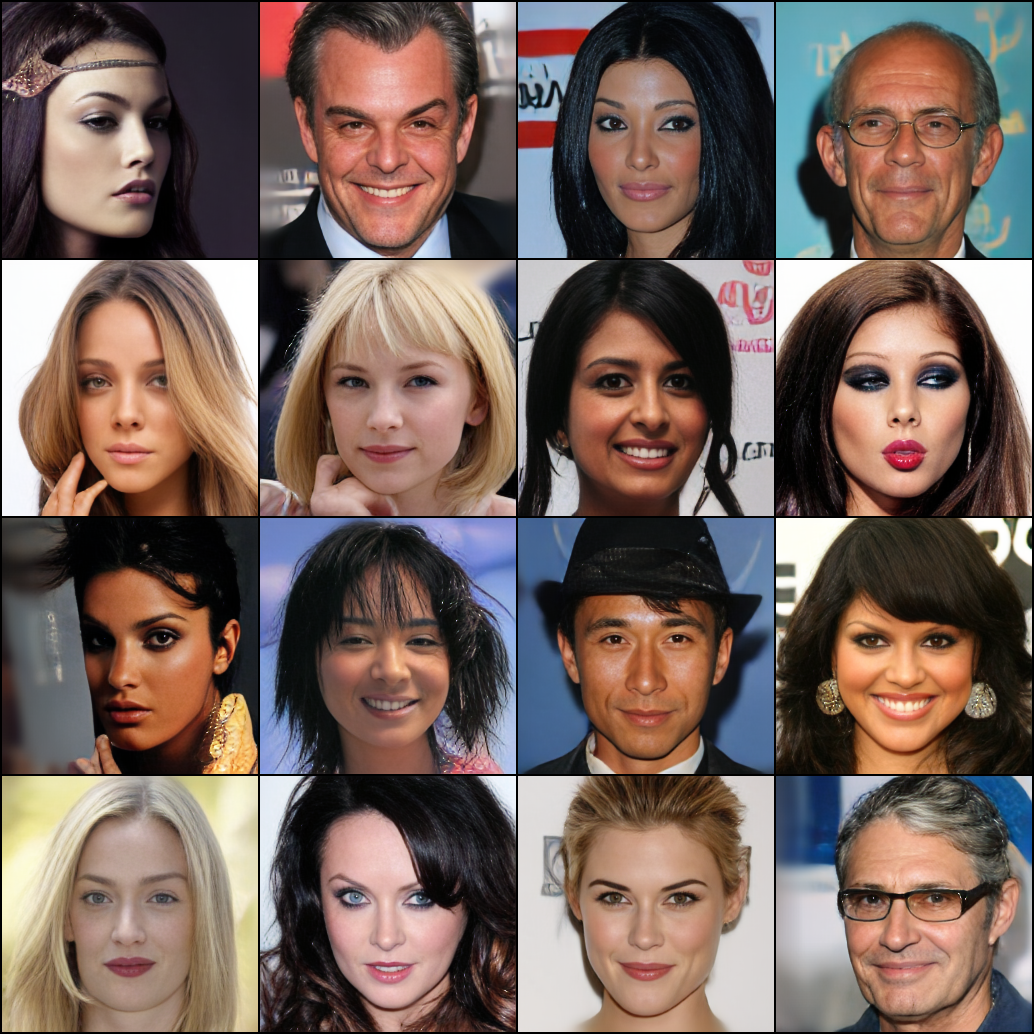
\includegraphics[width=0.47\linewidth]{celebahq_powerlong_stage2_samples_4x4_02.png} \\
        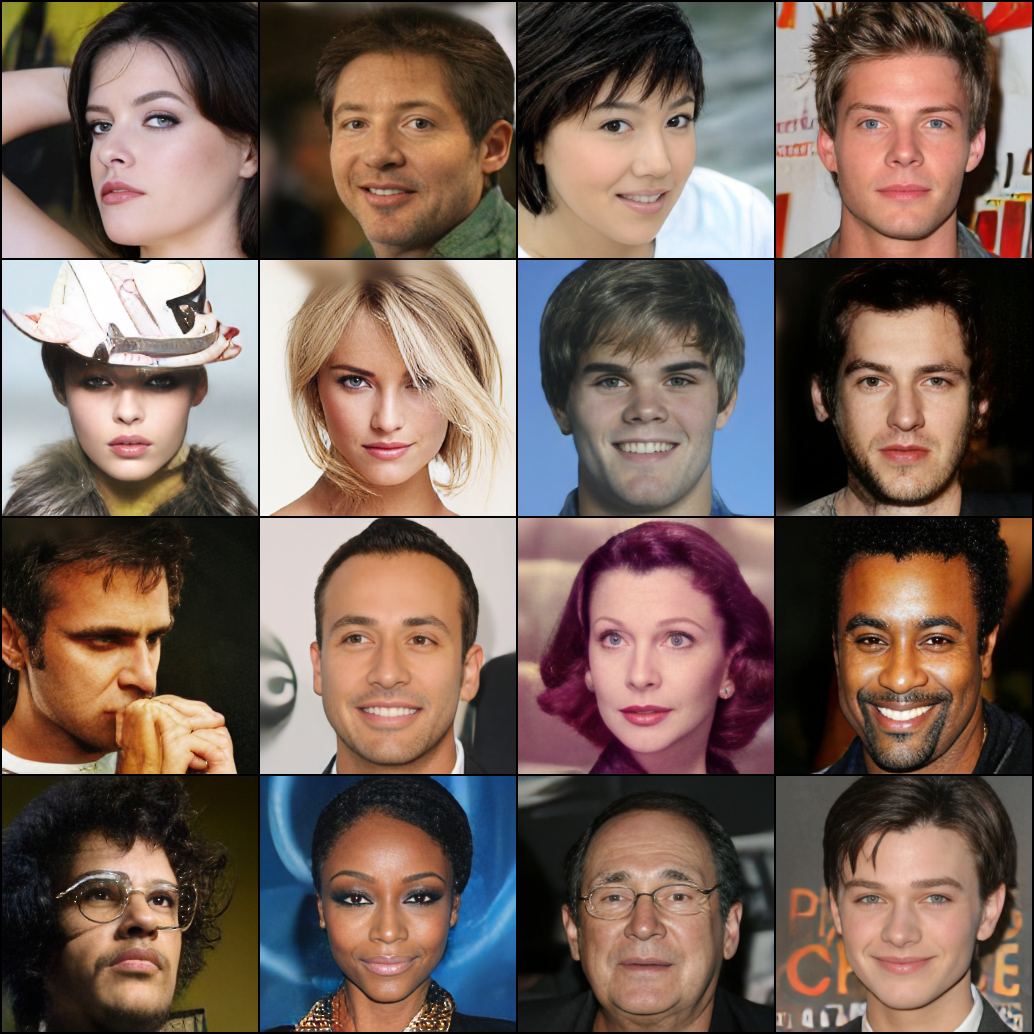
\includegraphics[width=0.47\linewidth]{celebahq_powerlong_stage2_samples_4x4_03.png} &
        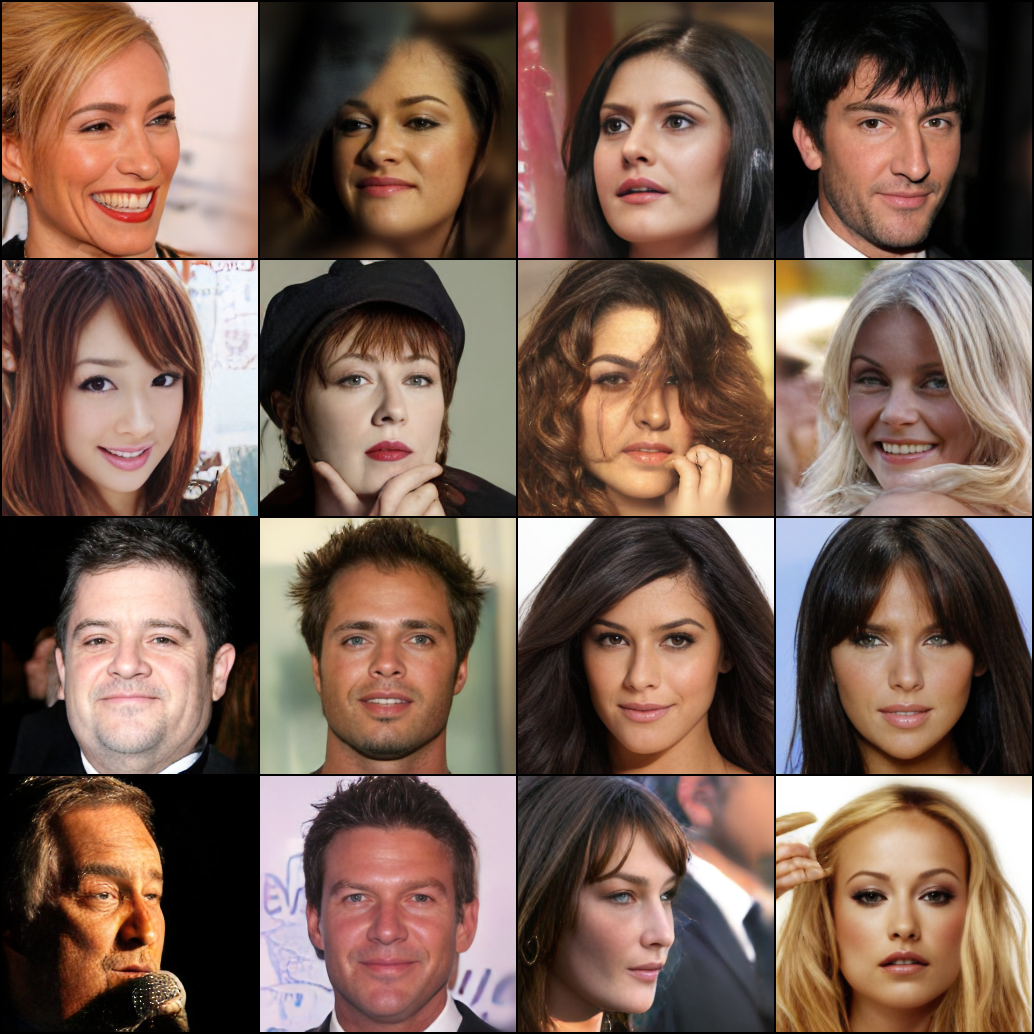
\includegraphics[width=0.47\linewidth]{celebahq_powerlong_stage2_samples_4x4_04.png}
    \end{tabular}
    \caption{Four $4 \times 4$ CelebA-HQ sample crops from the reported stage-2 prior.}
    \label{fig:celebahq-powerlong-samples}
\end{figure}

\FloatBarrier

\subsection{VCTK Waveform Audio Results}

The VCTK setting models raw waveform segments with the sparse dictionary bottleneck described above. Mel loss is disabled, so this experiment tests whether the sparse-token interface can support waveform reconstruction and generation without relying on mel-domain supervision. We report the audio results qualitatively through waveform traces, mel-spectrogram diagnostics, and generated waveform samples.

The non-adversarial and adversarial stage-1 variants both preserve the temporal structure of validation speech clips after sparse dictionary compression and decoding. The corresponding audio stage-2 transformer generates waveform clips from sparse-token sequences decoded through the learned waveform autoencoder. Qualitatively, these generated clips are human-sounding and have speech-like waveform envelopes.

\begin{figure}[!htbp]
    \centering
    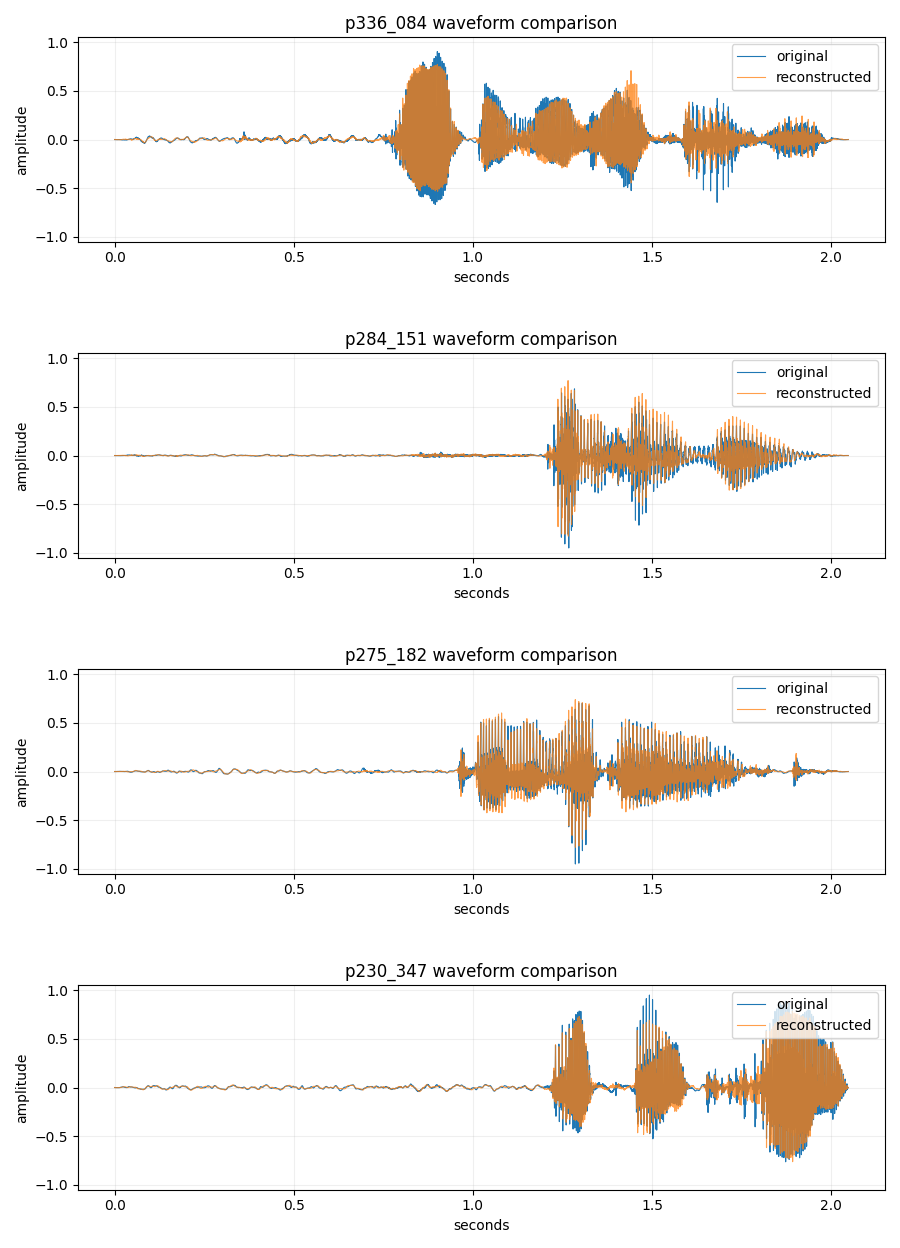
\includegraphics[width=0.88\linewidth]{vctk_laser_val_waveforms.png}
    \caption{VCTK validation waveform comparisons from the non-adversarial LASER waveform model. Blue traces are source waveforms and orange traces are stage-1 reconstructions.}
    \label{fig:vctk-waveform-comparisons}
\end{figure}

\begin{figure}[!htbp]
    \centering
    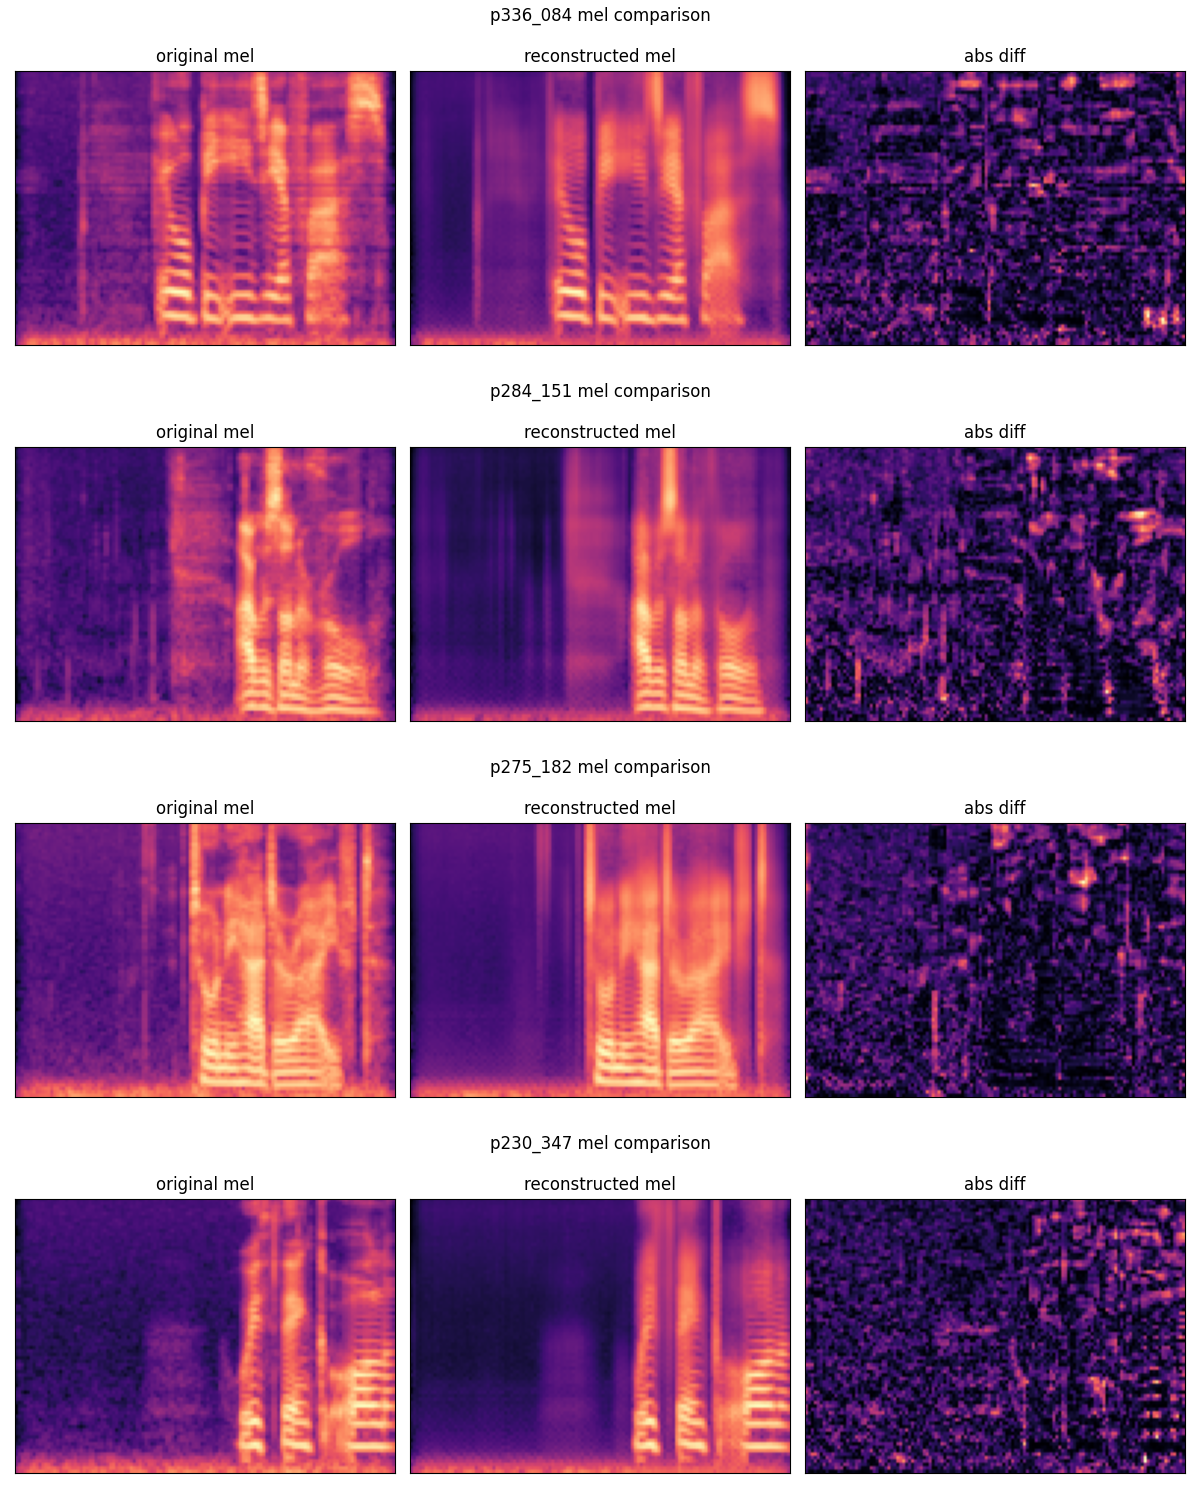
\includegraphics[width=0.98\linewidth]{vctk_laser_val_mels.png}
    \caption{VCTK validation mel-spectrogram diagnostics from the non-adversarial LASER waveform model. Each row shows original mel, reconstructed mel, and absolute difference.}
    \label{fig:vctk-mel-comparisons}
\end{figure}

\begin{figure}[!htbp]
    \centering
    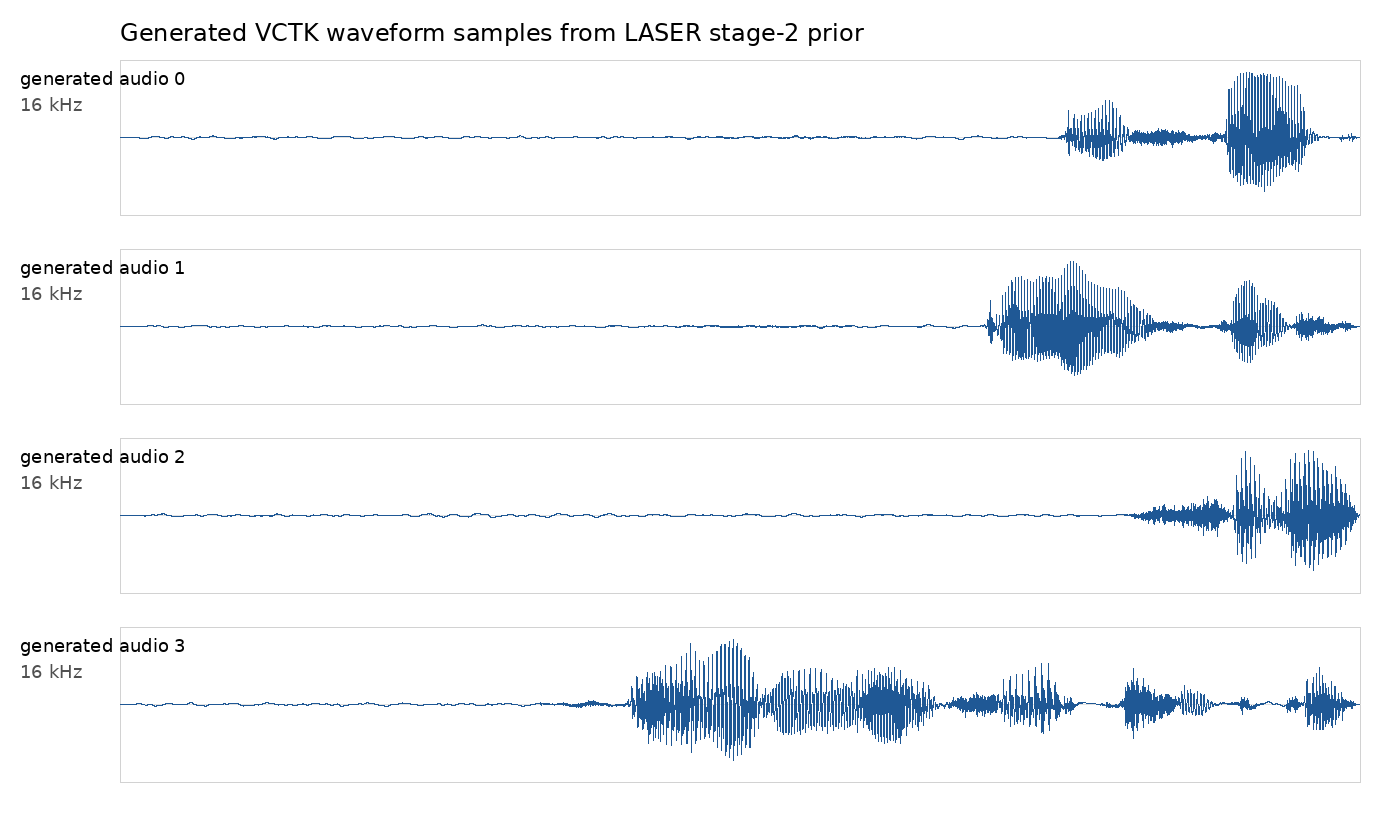
\includegraphics[width=0.98\linewidth]{vctk_laser_generated_waveforms.png}
    \caption{Generated VCTK waveform samples from the LASER stage-2 prior. The samples are generated from sparse-token sequences and decoded through the waveform stage-1 model.}
    \label{fig:vctk-generated-waveforms}
\end{figure}

\begin{figure}[!htbp]
    \centering
    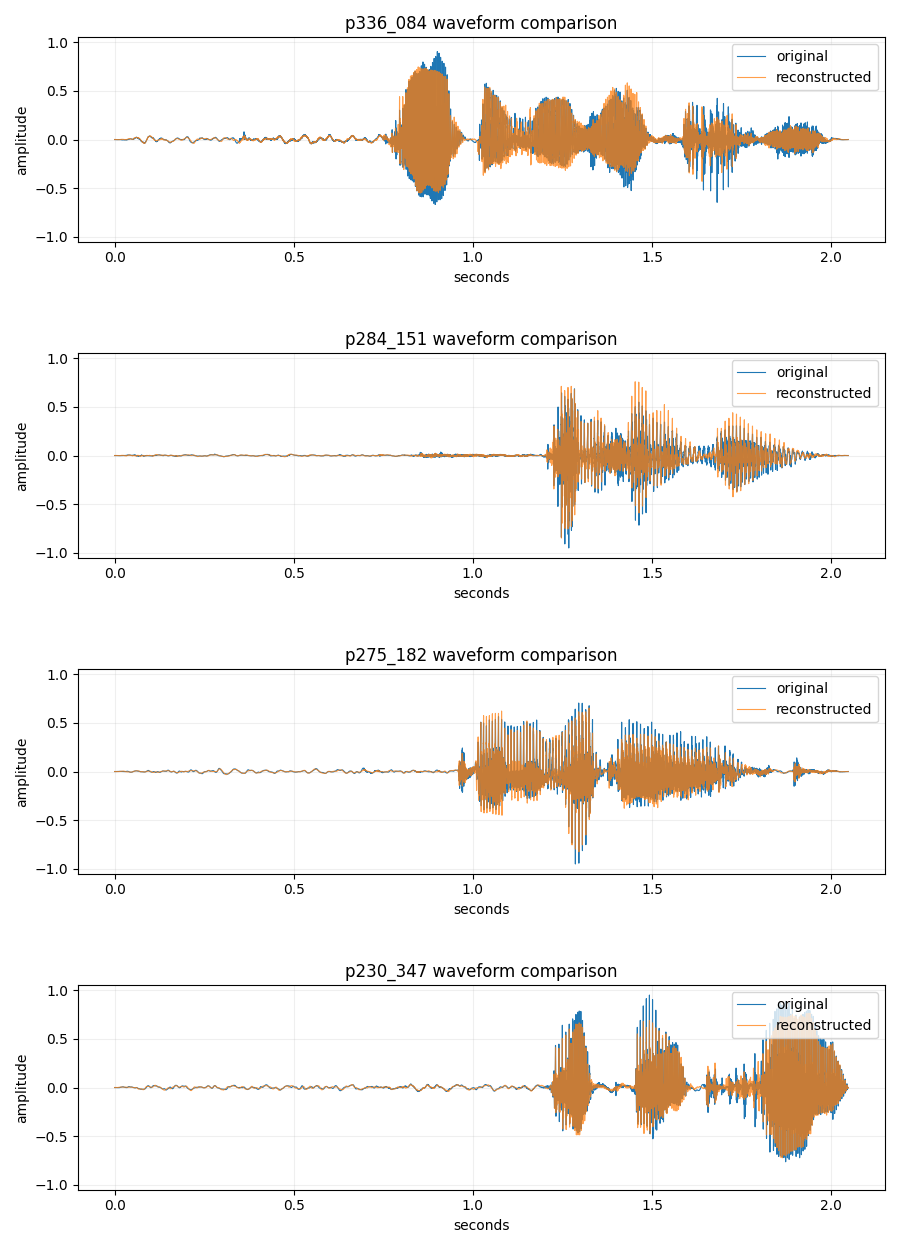
\includegraphics[width=0.88\linewidth]{vctk_laser_adv_val_waveforms.png}
    \caption{VCTK validation waveform comparisons from the adversarial LASER waveform model. Blue traces are source waveforms and orange traces are reconstructions.}
    \label{fig:vctk-adv-waveform-comparisons}
\end{figure}

\begin{figure}[!htbp]
    \centering
    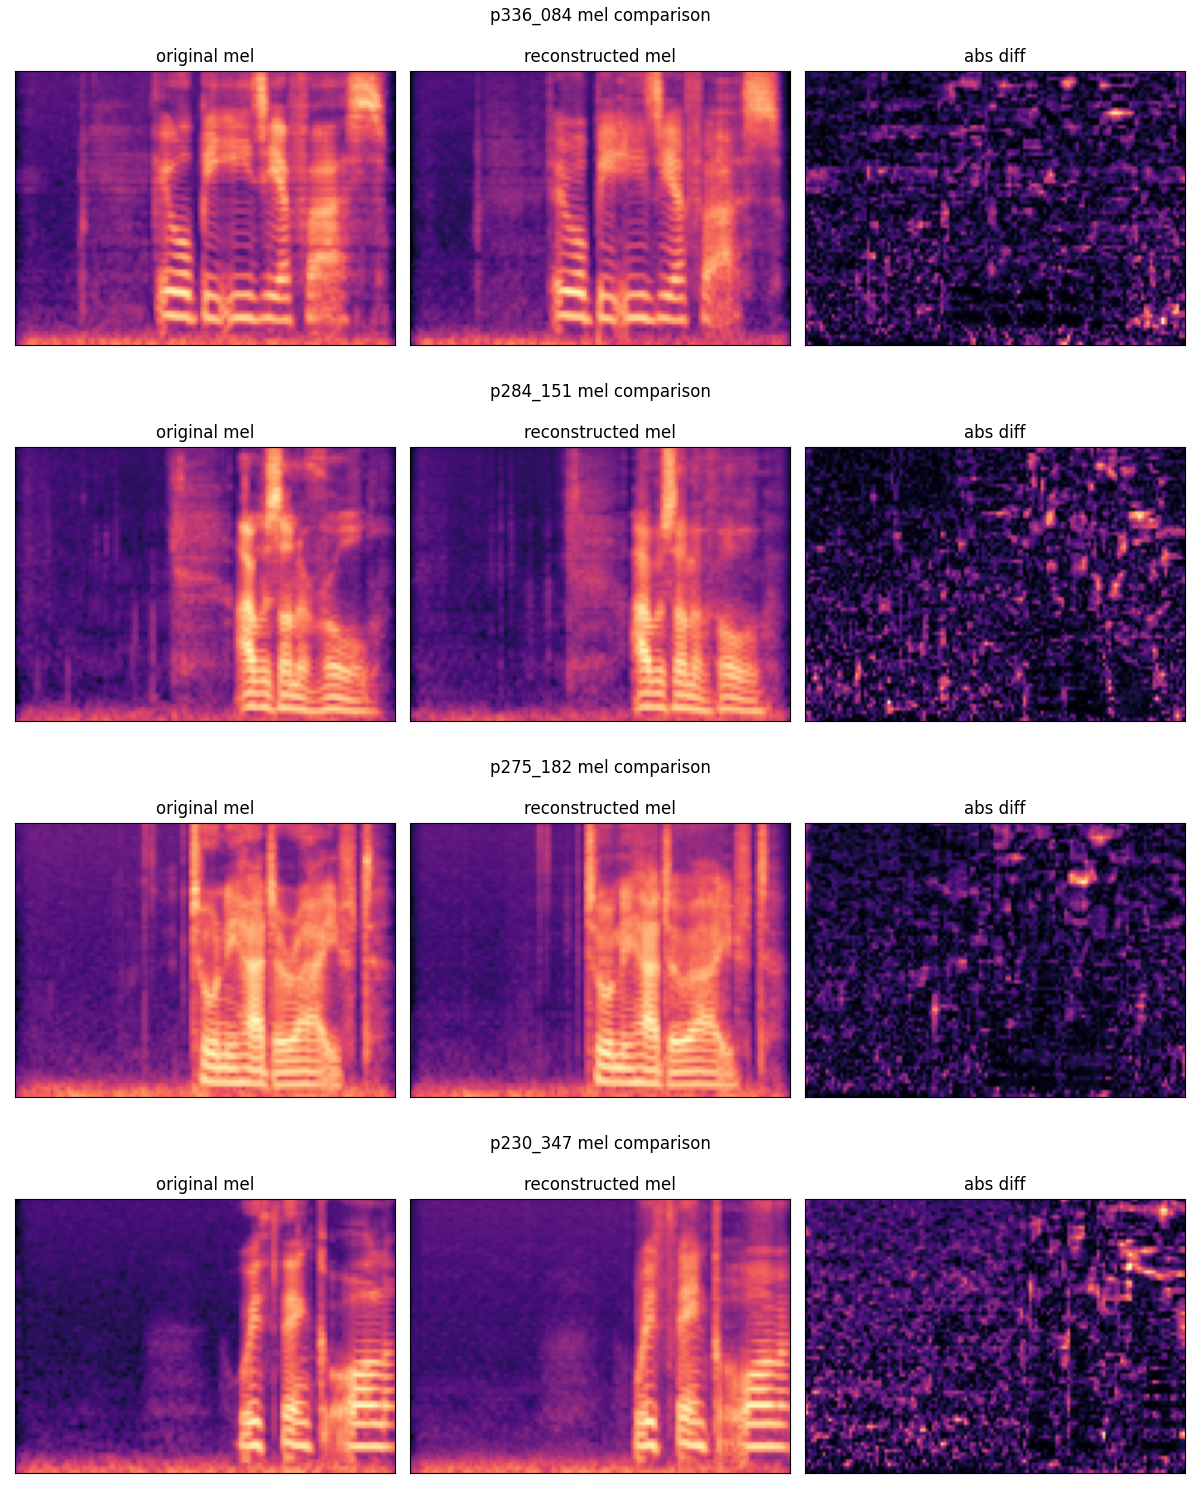
\includegraphics[width=0.98\linewidth]{vctk_laser_adv_val_mels.png}
    \caption{VCTK validation mel-spectrogram diagnostics from the adversarial LASER waveform model. Each row shows original mel, reconstructed mel, and absolute difference.}
    \label{fig:vctk-adv-mel-comparisons}
\end{figure}

\FloatBarrier

\section{Discussion}

The experiments support the central claim of the paper: useful generative latents do not have to be structured as one discrete codebook entry per site. LASER imposes a sparse dictionary structure instead, so each local latent is represented by a compact combination of learned atoms. The CelebA-HQ reconstruction and helper visualizations show that this bottleneck can preserve meaningful image structure while producing sparse, interpretable latent activity. The adversarial stage-1 continuation further improves the reconstruction distribution measured by rFID, and the stage-2 samples show that the resulting sparse-token representation can be modeled by an autoregressive prior.

The VCTK waveform results reinforce the same point in a different modality. The model uses the same sparse-token interface for raw audio, with modality-specific encoder, decoder, and reconstruction terms. The waveform and mel-spectrogram diagnostics indicate that the dictionary bottleneck preserves speech structure, and the generated stage-2 clips are human-sounding in qualitative listening inspection. This suggests that the sparse representation is not merely an image-specific construction, but a general way to impose compressive structure on latent spaces.

More broadly, these results suggest that the success of VQ-style generative modeling should not be attributed only to discreteness. Discretization is important for token-based priors, but it is only one part of the modeling story. The latent space must first be organized into a useful compressed representation. Dictionary learning provides one such organization by replacing a finite set of isolated prototypes with a union of low-dimensional subspaces. This gives the model a compositional latent geometry while still allowing the sparse codes to be quantized for sequential generation.

\section{Limitations}

The goal of this paper is to propose and validate an idea for structuring latent spaces, not to claim state-of-the-art performance. Sparse dictionary learning is one effective compressive structure, but it is not the only possible one. Other lossy compression mechanisms may induce different latent geometries with different tradeoffs, and exploring this broader design space is a natural direction for future work.

The reported transformer prior is also intentionally simple. Its role is to demonstrate that tokenized sparse codes can support sequential generation after the dictionary bottleneck has learned a compact representation. A more heavily optimized autoregressive model, sampling scheme, or likelihood objective may improve generation quality, but that architecture search is separate from the latent-structure claim. Finally, the sparse-coding step introduces some computational overhead and relies on a fixed sparsity choice; these are practical tradeoffs of using a union-of-subspaces bottleneck rather than a single nearest-neighbor codebook assignment.

\section{Related Work}

\paragraph{VQ-family models.}
Variational autoencoders with a discretization bottleneck, including VQ-VAE~\citep{oord2017vqvae} and VQGAN~\citep{esser2021vqgan}, provide compressed latent spaces that can be modeled by autoregressive priors. These models demonstrate that a learned compression bottleneck can be highly effective for generation. LASER follows the same broad two-stage philosophy, but replaces the finite-codebook geometry with sparse dictionary learning.

\paragraph{Sparse coding and dictionary learning.}
Sparse dictionary learning has a long history as a signal representation technique~\citep{olshausen1997sparse,aharon2006ksvd,tropp2007omp}. The main difference in LASER is that the dictionary is learned as part of a deep generative autoencoder, and the resulting sparse codes are explicitly tokenized for a second-stage prior. In this sense, LASER is not only a reconstruction model but also a latent-tokenization mechanism for generative modeling.

\paragraph{Transformer priors.}
Autoregressive transformers~\citep{vaswani2017attention} are a natural choice for modeling discrete latent tokens. VQ models typically provide one token per latent site, while RQ-Transformer~\citep{lee2022rqvae} models residual-quantized code stacks with a spatial-depth factorization. LASER adopts the same factorization for sparse support/coefficient token stacks, separating spatial context from the local sparse tuple at each site.

\section{Conclusion}

In this paper, we have examined the effectiveness of structuring latent spaces with sparse dictionary learning. LASER replaces a single discrete latent code with a sparse dictionary representation and then tokenizes the support and coefficient values for transformer-based generation. The CelebA-HQ results show strong image reconstruction and sparse-prior training behavior for a working instance of the model. The VCTK results show that the same two-stage sparse-token interface extends to raw waveform audio. These results suggest that discretization is not the only route to effective latent representations, and that lossy compression methods from signal representation can provide useful structure for modern generative models.

\bibliography{refs}
\bibliographystyle{tmlr}

\end{document}
